\documentclass{beamer}
\usepackage{progressbar, tcolorbox, CJKutf8, hyperref, multicol, pdfpages, graphicx, xcolor, blindtext, tikz, pgfplots, listings, smartdiagram}
\usepackage[absolute,overlay]{textpos}
\usepackage[backend=bibtex,style=numeric,sorting=none]{biblatex}

\hypersetup{
    colorlinks=true,
    linkcolor=blue,
    filecolor=magenta,      
    urlcolor=blue,
    }

\definecolor{mygreen}{rgb}{0,0.6,0}
\definecolor{mygray}{rgb}{0.5,0.5,0.5}
\definecolor{mymauve}{rgb}{0.58,0,0.82}

  \lstset{ 
  backgroundcolor=\color{white},   % choose the background color; you must add \usepackage{color} or \usepackage{xcolor}; should come as last argument
  basicstyle=\ttfamily\footnotesize,% the size of the fonts that are used for the code
  breakatwhitespace=false,         % sets if automatic breaks should only happen at whitespace
  breaklines=true,                 % sets automatic line breaking
  captionpos=b,                    % sets the caption-position to bottom
  commentstyle=\color{mygreen},    % comment style
  deletekeywords={...},            % if you want to delete keywords from the given language
  escapeinside={\%*}{*)},          % if you want to add LaTeX within your code
  extendedchars=true,              % lets you use non-ASCII characters; for 8-bits encodings only, does not work with UTF-8
  frame=single,	                   % adds a frame around the code
  keepspaces=true,                 % keeps spaces in text, useful for keeping indentation of code (possibly needs columns=flexible)
  keywordstyle=\color{magenta},        % keyword style
  morekeywords={FROM, RUN, ENV, USER, WORKDIR, CMD, EXPOSE, ADD, COPY, sudo, curl, chmod, ln, git, cd},
                                   % if you want to add more keywords to the set
  numbers=left,                    % where to put the line-numbers; possible values are (none, left, right)
  numbersep=5pt,                   % how far the line-numbers are from the code
  numberstyle=\tiny\color{mygray}, % the style that is used for the line-numbers
  rulecolor=\color{black},         % if not set, the frame-color may be changed on line-breaks within not-black text (e.g. comments (green here))
  showspaces=false,                % show spaces everywhere adding particular underscores; it overrides 'showstringspaces'
  showstringspaces=false,          % underline spaces within strings only
  showtabs=false,                  % show tabs within strings adding particular underscores
  stepnumber=1,                    % the step between two line-numbers. If it's 1, each line will be numbered
  stringstyle=\color{mymauve},     % string literal style
  tabsize=4,	                     % sets default tabsize to ˋ spaces
  title=\lstname
}

\graphicspath{ {./images/} }
\usetheme{AnnArbor}
\addbibresource{main.bib}
\usetikzlibrary{positioning, calc, shapes.multipart, shapes.arrows, fit, backgrounds}

\definecolor{dockerColor}{RGB}{13, 183, 237}
\definecolor{secureColor}{RGB}{10, 191, 83}
\definecolor{aquamarine}{rgb}{0.5, 1.0, 0.83}
\definecolor{aquamarine2}{rgb}{0.2, 1.0, 0.53}

\title{The Container Security in Healthcare Data Exchange System}
\subtitle{Bachelor's degree graduation project}
\author{Chih-Hsuan Yang}
\institute{National Sun Yat-sen University\\
Advisor: Chun-I Fan
}
\date{\today}

\AtBeginSection[]{
  \begin{frame}
  \vfill
  \centering
  \begin{beamercolorbox}[sep=8pt,center,shadow=true,rounded=true]{title}
    \usebeamerfont{title}\insertsectionhead\par%
  \end{beamercolorbox}
  \vfill
  \end{frame}
}



\begin{document}
\begin{CJK*}{UTF8}{bsmi}

  \begin{frame}
    \titlepage
  \end{frame}


  \begin{frame}{Outline}
    \begin{multicols}{2}
      \tableofcontents
    \end{multicols}
  \end{frame}

  \section{stavhaygn}
  \begin{frame}{Analyzing}
    \begin{enumerate}
      \item LSM calling sequence of syscall
            \begin{itemize}
              \item \href{https://github.com/quark-engine/quark-engine}{Quark-Engine}, Bayes' theorem
              \item Difficulty
                    \begin{enumerate}
                      \item Hard to specify which app on witch container (context switch)
                      \item Generating rules
                      \item False positive is really severe
                    \end{enumerate}
            \end{itemize}
      \item Check the image
            \begin{itemize}
              \item Check the signature and hash?
              \item Native \href{https://docs.docker.com/engine/scan/}{docker scan} supports.
              \item Scan apps in layers.
            \end{itemize}
    \end{enumerate}
  \end{frame}

  \begin{frame}
    \centering
    \begin{multicols*}{2}
      % \begin{beamerboxesrounded}
      \lstinputlisting[basicstyle=\tiny, numbers=left]{src/Dockerfile}
      % \end{beamerboxesrounded}
      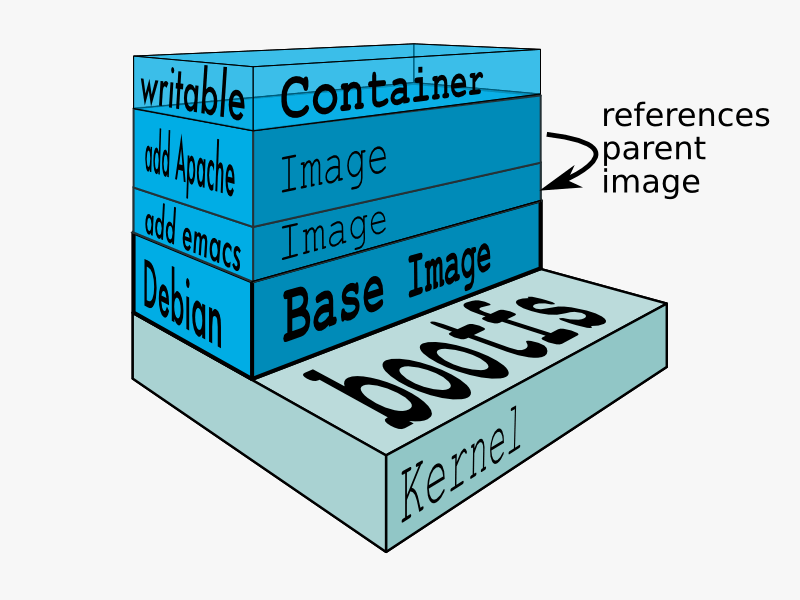
\includegraphics[width=.45\textwidth]{layers.png}
    \end{multicols*}
  \end{frame}

  \begin{frame}
    \centering
    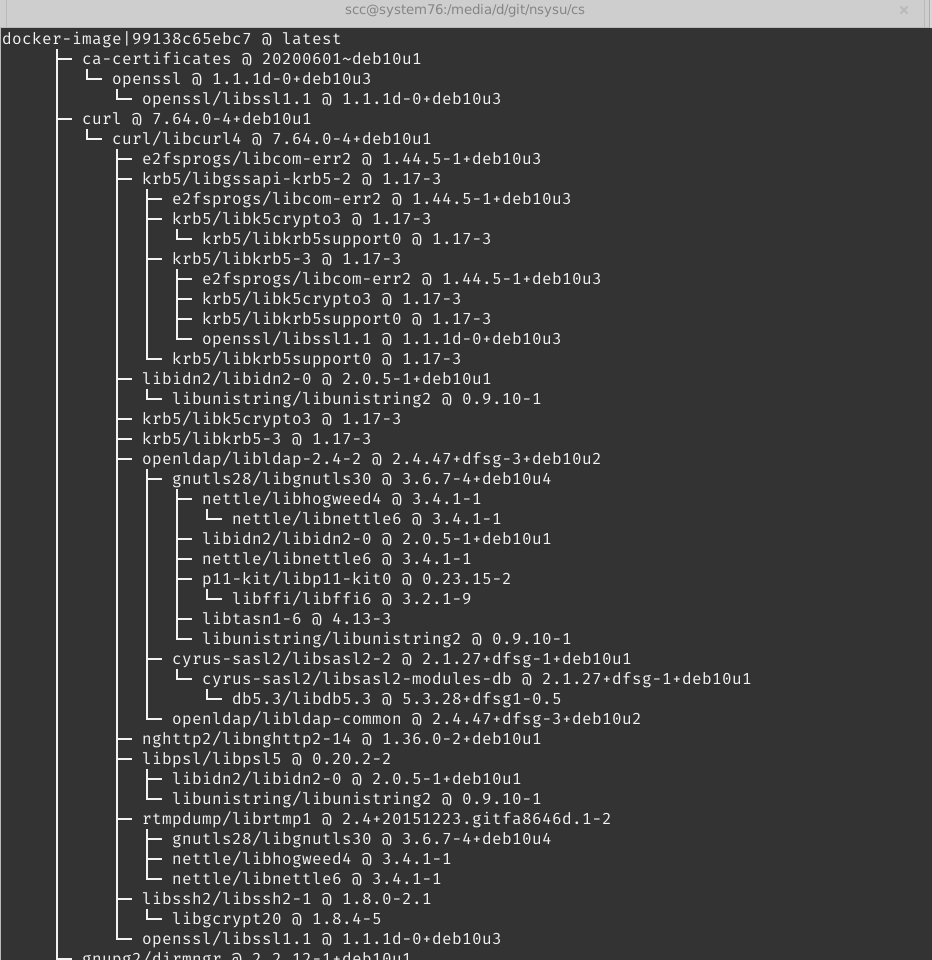
\includegraphics[height=\textheight]{Screenshot_2021-07-23_12-02-42.png}
  \end{frame}

  \section{Tim}
  \begin{frame}{Share the kernel}
    \begin{itemize}
      \item Mixed: configuration and rule based
      \item built time to whitelist of syscall
    \end{itemize}
  \end{frame}

  \begin{frame}{Idea and compare}

    \begin{itemize}
      \item The false positive and false negative rate.
      \item Maybe I can mix this two mechanism together.
    \end{itemize}
    Compare to others mechanism?
  \end{frame}

  \begin{frame}{Flow chart}
    \centering
    \scalebox{0.9} {
      \smartdiagram[flow diagram:horizontal]{
        Scan base, Sign, Image checking, Start policy, Runtime enforcement
      }
    }
  \end{frame}

  {
  \setbeamertemplate{navigation symbols}{}
  \begin{frame}[plain]
    \makebox[\linewidth]{
\includegraphics[width=\paperwidth]{rust_linux.jpg}}
    \centering
    \href{https://min.news/en/tech/6a15a93324c35f2e4c26213dfe04431d.html?__cf_chl_jschl_tk__=pmd_fae7f5a25085221cdd53313705eb12bc13a31bb7-1627020947-0-gqNtZGzNAk2jcnBszQai}
    {Write kernel module in Rust}
  \end{frame}
  }

  % \begin{frame}{References}
  %   \def\bibfont{\footnotesize}
  %   \printbibliography
  % \end{frame}

\end{CJK*}
\end{document}